\chapter{Formal model}
\label{chap:model}
We aim to show the importance of dissemination and verification of interactions 
records. This is done by defining a model within which we can prove that record
dissemination and verification are essential for securing the trust system. Also we define a
mechanism which allows to protect the network against free-riders which 
jeopardize the overall security. Our proposal is to introduce exchange transparency which can 
effectively punish free-riders that do not acquire and disseminate interaction records. We further 
show that it is possible to detect agents that consciously interact with malicious agents, exposing
them as verification free-riders or accomplices.

\section{Model definition}
\label{sec:definitions}
We make use of the ordered interaction model which has been introduced in previous work from 
our research group by Otte et. al. in \cite{OTTE2017}. We restate it in Definition \ref{def:old_base} for clarity.
The symbols were annotated in order to reuse symbols in later definitions.

\begin{defn}[Ordered interaction model]. 
    \label{def:old_base}
    An ordered interaction model $\hat M = \langle \hat P, \hat I, \hat a, \hat w \rangle$ consists of two sets and two 
    functions.
    \begin{itemize}
        \item $\hat P$, a finite set of agents
        \item $\hat I$, a finite set of interactions
        \item $\hat a : I \rightarrow P \times P$, a function mapping each interaction to the agents 
        involved in it.
        \item $\hat w : I \times P \rightarrow \mathbb{R}_{\geq0}$, a function which describes the 
        contribution of an agent in an interaction
    \end{itemize}
\end{defn}

The model allows for the analysis of any type of application in which a network of agents performs
transactions that can be described by a quantitative amount. However, the model does not explicitly
model the information exchange between agents. Our goal is to show that in a distributed trust system this 
exchange of information is also an essential component to guarantee manipulation resistance. We 
therefore extend the model with this concept of exchange.

\begin{defn}[Ordered encounter model]. 
    \label{def:base}
    An ordered encounter model $M = \langle P, I, E, a, w, x \rangle$ is a 6-tuple consisting
     of three sets and three functions. For convenience we define a set $N = I \cup E$. 
    \begin{itemize}
        \item $P$, a finite set of agents
        \item $I$, a finite set of interactions
        \item $E$, a finite set of exchanges
        \item $a : N \rightarrow P \times P$, a function mapping each interaction and exchange to the agents 
        involved in it.
        \item $w : I \times P \rightarrow \mathbb{R}_{\geq0}$, a function which describes the 
        contribution of an agent in an interaction
        \item $x : E \times P \rightarrow N^+$, a function which describes the interactions that an 
        agent received in an exchange. $+$ refers to the Kleene plus.
    \end{itemize}
\end{defn}

Also it should be noted that for any $p \in P$, $i \in I$ and for which $p \notin a(i)$, $w(i,p) = 0$, 
and for any $e \in E$, if $p \notin a(e)$, then $x(e, p) = \emptyset$.
We call the set $N$ the encounters of the model. An encounter happens between two agents for one of
two reasons: to perform a transaction of some value or to exchange information.
Interaction in this model are the equivalent of transactions of value in an application context. 
An exchange on the other hand is a transaction of information about other encounters.
The function $x$ describes a set of encounters that an agent obtains through an 
exchange. Gossiping, that is the exchange of information with a random peer, is one way to create 
such exchanges. We will formally introduce the 
knowledge concept in Definition~\ref{def:subjective_network_state}.

For each agent we can describe the set of encounters which that agent participated in as the agent 
encounter history. 

\begin{defn}[Agent encounter history]
    Given an ordered encounter model $M = \langle P, I, E, a, w, x \rangle$ the agent encounter history of an agent $p \in P$ is defined as follows:
    \begin{equation}
        H_p = \{ n \in N : p \in a(n) \}
    \end{equation}
\end{defn}


The history of an agent $p$ is totally ordered by $<$. If we denote the 
$t$th encounter of $p$ as $n_p(t)$ then we can alternatively write $N_p = \{ n_p(1), n_p(2), ..., n_p(i)\}$.

Encounters between agents are not public. This creates a discrepancy between the true set of 
encounters $N$ and the observed encounters from an agent $p$'s point of view. Agents only have 
knowledge of those encounters which they participated in or which they obtained knowledge of through an exchange.
We can then define the subjective network state, which is the knowledge an agent has about the state of
the network.

\begin{defn}[Subjective network state]
    \label{def:subjective_network_state}
    Given an ordered encounter model $M = \langle P, I, E, a, w, x \rangle$ and an agent $p \in P$ with encounter history $H_p$, the subjective network state of agent $p$
    is defined as follows:
    \begin{equation}
        N_p = H_p \cup \{ x(e, p) : e \in E \text{ and } e \in H_p \}
    \end{equation}
\end{defn}

The subjective network state contains the complete knowledge of the agent. In \cite{OTTE2017} a 
similar concept exists in the form of the subjective work graph. It generally models a partial view
of the network described by the model. This subjective view is the basis for the calculation of 
reputation and trust as further described by Otte et.al.. At the core of this work is not the way 
reputation and trust are calculated but rather how the knowledge of interactions is disseminated and
protected against malicious agents. The relation to actual trust creation is further discussed in 
Section \ref{sec:relevance}

The model from Definition \ref{def:base} introduces the concept of exchanges. Yet it does not define
how agents should exchange data. We therefore define an exchange policy which is the strategy that 
honest agents apply for exchanging information.

\begin{defn}[Exchange policy]
    Given an ordered encounter model $M = \langle P, I, E, a, w, x \rangle$ and an agent $p \in P$ with encounter history $N_p$,
    the exchange policy is a function $f : I_p \rightarrow P \times N^+$, where $I_p = \{ n \in N_p  \cap I\}$.
    The exchange policy maps each interaction of an agent $p$ to a partner and set of encounters 
    which need to be obtained from that partner prior to the interaction.
\end{defn}

The exchange policy defines which information an agent needs to have in order for an interaction to 
be valid. This is to ensure that an agent has all the information to ensure that the partner is also
an honest agent. It should be noted that an honest agent has no reason not to reply to an exchange 
request. 

As the exchanges are recorded it is possible to determine whether an agent adheres to a certain 
exchange policy. 

\begin{defn}[Exchange policy adherence]
    Given an ordered encounter model $M = \langle P, I, E, a, w, x \rangle$ and the history $H_p$ of an
    agent $p$, the condition for adhering to a policy $f$ and
    therefore being considered an honest agent is as follows: 

    \begin{equation}
        f(I_p) \subseteq \{ (q, x(e, p)) : e \in H_p \cap E,  \exists (p, q) \in a(e)\}
    \end{equation}
\end{defn}

% The subjective network state also implies the known agents $P_p = \{ q \in P : n \in N_p, q \in a(n) \}$
% Without full observability there is also no guarantee that agents know the full history of their 
% peers. Actually the subjective network state defines also $p$'s observed peer history of an agent $q$.

% \begin{equation}
%     H_{p, q} = \{ n \in N_p : q \in a(n) \}
% \end{equation}

% Similar the observed peer history is a totally ordered set. It is not necessarily equal to the 
% complete history though. For example, an agent $q$'s history $H_{q} = \{n_q(1), n_q(2), n_q(3) \}$
% could be observed by an agent $p$ as $H_{p, q} = \{n_q(1), n_q(3)\}$.

% Finally, a reputation mechanism needs to be defined. Agents estimate the reputation of their peers
% from their subjective network state. 

% \begin{defn}[Reputation mechanism] 
%     A reputation function $R$ takes as input the subjective network state $N_{p}$ and determines 
%     a reputation score $S^R_{p,q}(I_{p,q}) \in \mathbb{R}$ for all known agents $P_p$.
% \end{defn}

\section{Fork and double spend defense}
\label{sec:model_double_spend}
In what follows we analyze the defense of certain exchange policies against a double spend attack. 
That attack is a potent attack on a network that can be modelled by an ordered encounter model. 
Conceptually, an attacker 
has two conflicting interactions at the same time with two different agents. As each partner is not
aware of the other both accept the interaction. 

\begin{defn}[Fork and double spend]. Given an ordered encounter model $M = \langle P, I, E, a, w, x \rangle$, a malicious agent $p$ has two conflicting interactions 
    $i \in I$ and $j \in I$ at the exact same time such that $i = n_p(t)$ and $j = n_p(t)'$. Both interactions have a different partner $a(i) = (p, q)$ 
    and $a(j) = (p, r)$. Accordingly, the history  of $p$ is not a totally ordered set anymore.
    The attack can be detected if for any honest agent $s$, $i \in N_{s}$ and $j \in N_{s}$ are
    true.
\end{defn}

In the following we show that exchanging blocks is essential for the network to defend against such an 
attack. We first study the case of no exchanges. For that we formally define the No-Exchange policy.

\begin{pol}[No-Exchange]
    \label{pol:no-exchange}
    The No-Exchange policy defines no required exchanges for an honest agent, so $f(I_p) := \emptyset$.
\end{pol}

Without any exchanges, agent are only aware of the interactions that they perform themselves. In
Figure \ref{fig:no_exchange_policy} we consider a situation in which five honest agents perform interactions. 
The timeline of each agent is represented by the horizontally dashed line. Each interaction is 
connected to two agents' timelines. The No-Exchange policy requires no exchanges so agents only have
interactions. Each connected interaction is part of an agent's history. The figure indicates with 
blue, the blocks that agent F is aware of which are only those he participated in.

\begin{figure}
    \centering
    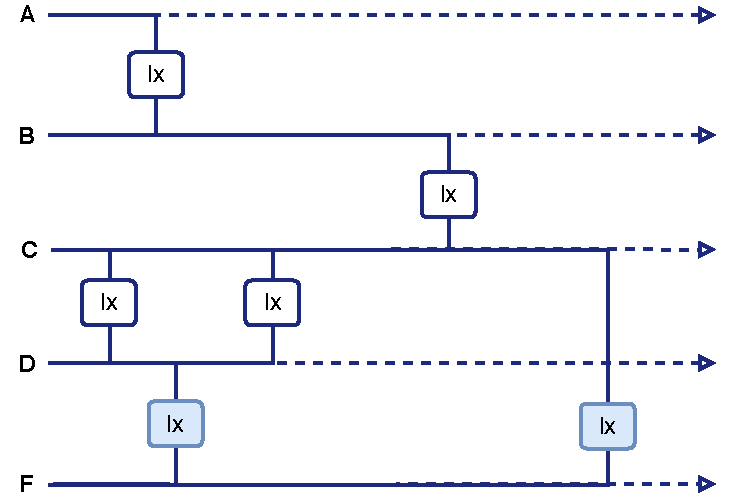
\includegraphics[width=0.5\textwidth]{images/no_exchange_policy.pdf}
    \caption{History graph of No-Exchange policy in our model. We consider 5 agents. Each agent has a time
    line which is connected to interactions(denoted by Ix). Each interaction is between two agents. The blue blocks show the subjective network state of agent F.}
    \label{fig:no_exchange_policy}
\end{figure}

\begin{thm}[Detectability of double spend without exchanges]
    \label{thm:fork_no_gossiping}
    If honest agents apply the No-Exchange policy, the fork and double spend attack cannot be detected.
\end{thm}
\begin{proof}
    Let $p$ be the attacking agent and let $i$ and $j$ be the conflicting interactions of the 
    attacks. Further, let $q$ be the partner in interactions $i$ such that $a(i) = (p, q)$ and let 
    $r$ be the partner of interaction $j$ such that $a(j) = (p, r)$. 
    The No-Exchange policy implies that for any honest agent $s \in P$ and all $e \in E$, $x(e, s) = \emptyset$ 
    and therefore $N_s = H_s$ applies. 
    According to Definition \ref{def:subjective_network_state} $i \in N_{q}, j \notin N_{q}$ and 
    $i \notin N_{r}, j \in N_{r}$. 
    Furthermore, for any honest $s \in P$, $i \notin N_s$ and $j \notin N_s$ must be true because
    $s \notin a(i)$ and $s \notin a(j)$.
    % Without gossiping both $q$ and $r$ will not further disseminate 
    % their interactions with $p$ and therefore will not learn of the other version.
    % Moreover, all other agents $s \in P$ are aware of neither $i$ or $j$ because only direct 
    % interactions are observed. Consequently no agent observes both $i$ and $j$.
\end{proof}

Theorem \ref{thm:fork_no_gossiping} proves that the double spend attack cannot be
detected without exchanging encounters. 

We now show that if agents do exchange information, this can lead to the detection of the attacker. We
define an exchange policy in which honest agents obtain the encounter history prior to an interaction.

\begin{pol}[History-Exchange policy]
    \label{pol:one}
    The History-Exchange policy requires agents to obtain the encounter history of their partner 
    prior to an interaction. 

    \[ f(I_p) := \{ (q, H_q) : \exists i, q (i \in I_p \text{ and } (p, q) \in a(i)) \}\]
\end{pol}

Figure \ref{fig:chain_exchange} shows the same 5 agents, with the same interactions. This time agents
apply the History-Exchange policy, which requires the exchange of both agents' histories prior to 
an interaction. The colored interactions and exchanges are received by F, green being those received
from D and purple those received from C. At the end of the shown timeline, the colored blocks are 
the subjective network state of F.

\begin{figure}
    \centering
    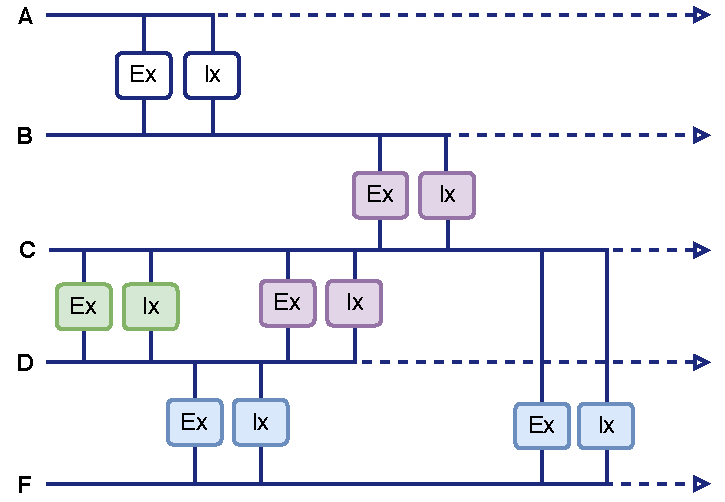
\includegraphics[width=0.5\textwidth]{images/chain_exchange.pdf}
    \caption{History graph of History-Exchange policy in our model. We again consider 5 agents. The 
    colored blocks show the subjective network state of agent F. The blue blocks are F's own encounters,
    the green block is an encounter received from D while the purple blocks are received from C.}
    \label{fig:chain_exchange}
\end{figure}

\begin{thm}[Detectability of double spend with the History-Exchange policy]
    \label{thm:fork_gossiping}
    If all honest agents apply the History-Exchange policy and periodically use uniform sampling over
    the set of agents to find an interaction partner, the double spending will eventually be detected.
\end{thm}
\begin{proof}
    Let $p$ be the attacking agent and let $i \in I$ and $j \in I$ be the conflicting interactions 
    of the attack at time $t$. Further, let $q$ be the partner in interactions $i$ such that 
    $a(i) = (p, q)$ and let $r$ be the partner of interaction $j$ such that $a(j) = (p, r)$. 
    According to Definition \ref{def:subjective_network_state} $i \in N_{q}, j \notin N_{q}$ and 
    $i \notin N_{r}, j \in N_{r}$.

    We consider an honest agent $q$ sampling agents for an interaction. For network size $l = |P|$ the 
    probability of choosing partner $r$ in the first round is $1/l$. The probability for not having
    chosen $r$ in any of $k$ rounds is $(\frac{l-1}{l})^k$ and $\lim_{k\to\infty}(\frac{l-1}{l})^k = 0$.
    Given an infinite amount of time, $q$ therefore chooses $r$ for an interaction and because $q$ is honest 
    performs an 
    exchange $e$ prior. $j \in H_r$ and therefore $j \in x(e, q)$, which means that after exchange 
    $e$ $i \in N_q \text{ and } j \in N_q$. Therefore $q$ is able to detect the double spending.
\end{proof}

Theorem \ref{thm:fork_gossiping} shows that exchaning encounter information makes double spending detectable. Once a double
spender is detected by an agent it is possible to ignore them for future interactions. The amount 
of exchange rounds until detection depends on the exact policy of exchanging data and a deeper 
analysis is beyond the scope of this work.

\section{Exchange free-riding}
We now look at ways to incentivize information exchanges. At this point we have shown that a system in which 
interactions are only directly observable by the direct participants, an exchange mechanism like 
History-Exchange policy is essential to defend against the double-spending attack. 
Our aim is now to show that a reputation mechanism which takes into account the exchange behavior of 
agents defends the system against free-riders. 

If bandwidth and storage capacity are valuable resources for agents, data dissemination and their 
long-term storage come at a cost for agents. Therefore agents can attempt to free-ride and only 
interact without exchanging data. However if all agents would behave in that way the system loses 
the ability to defend itself against forks and double spending as shown in Theorem 
\ref{thm:fork_no_gossiping}. We will call those agents Exchange free-riders. 

% An honest agent should also be able to verify that other agents adhere to an exchange policy or not.

% \begin{lem}[Exchange policy adherence]
%     \label{lem:policy_adherence}
%     Given an ordered encounter model $M$ with exchange policy $D$, any agent $p$ that has observed 
%     the complete history $H_s$ of an agent $s$ can determine whether that agent adhered to policy 
%     $D$.
% \end{lem}
% \begin{proof}
%     Agent $p$ has observed the complete history of agent $q$, therefore $H_q \subseteq N_p$. Agent 
%     $p$ is then able to calculate the frequency of $q$'s exchanges as $f^D_q = \frac{|\{ n \in H_q : n \in E \}|}{|\{ n \in H_q : n \in I \}|}$,
%     the partners of exchanges $S^D_q = \{ a(n) \setminus q : n \in H_q \text{and} n \in E \}$ and the 
%     exchanged encounter $E^D_q = \{ x(n,q) : n \in H_q \text{and} n \in E \}$. Then $p$ can compare
%     the calculated values to the expected values defined by $D$. 
% \end{proof}

\begin{defn}[Exchange free-rider]
    \label{def:gos_free-rider}
    Given an ordered encounter model $M = \langle P, I, E, a, w, x \rangle$ with exchange policy $f$, an exchange free-rider $p \in P$ is an 
    agent whose exchange behavior does not fulfill the minimum requirements of policy $f$. That is, 
    $f(I_p) \nsubset \{ (q, x(e, p)) : e \in H_p \cap E, \exists (p, q) \in a(e)\}$.
\end{defn}

We now show that exchange free-riders can be detected by honest agents that apply the History-exchange
policy.

\begin{thm}[Detectability of exchange free-riders]
    \label{thm:gos_free-rider}
    Given an ordered encounter model $M = \langle P, I, E, a, w, x \rangle$ in which honest agents use the History-Exchange policy
    an exchange free-rider will be detected on the first interaction.
\end{thm}
\begin{proof}
    Assume agent $p$ is an honest agent and is about to interact with agent $q$. Because agent $p$
    uses Policy \ref{pol:one}, $p$ will request an exchange with $q$. That exchange will contain 
    $H_q$. If it does not $p$ will know that $q$ is a exchange free-rider. After a successful
    exchange $H_q \subseteq N_p$. In that case $p$ is able to check the condition for adherence to 
    the History-Exchange policy $f$ by $f(I_q) \subseteq \{ (q, x(e, p)) : e \in 
    H_q \cap E, \exists (p, q) \in a(e)\}$. If the condition is not true agent $p$ has found $q$ to be a
    exchange free-rider.
\end{proof}

The detectability of exchange free-riders as shown in \ref{thm:gos_free-rider} means that any 
honest agent is able to ignore the free-rider on the first interaction. This takes away any 
possibility for future interactions with honest agents. We conclude that through exchanging
information on the encounters of agents we can effectively defend against 
exchange free-riders.

\section{Verification free-riding}
\label{sec:verification_free-riding}
We have shown that double-spenders and exchange free-riders can both be detected. Yet in order to 
actually detect those attacks, agents need to perform verification of any encounters received 
through exchanges. We can define Algorithm \ref{alg:verify_exchange} which is run by all 
honest agents for each exchange in order to defend against double-spenders and exchange free-riders.

\begin{algorithm}
\caption{Exchange verification}\label{alg:verify_exchange}
\begin{algorithmic}[1]
\Procedure{verifyExchange}{}
\State {$p$: Honest agent, receiver of exchange}
\State {$q$: Agent, subject of verification}
\State {$H_q$ \leftarrow $q$'s encounter history}
\State {$N_p$ \leftarrow $p$'s subjective network state}
\ForAll{exchanges $e$ in $H_q$ }
\If {$e$ is not valid according the the exchange policy} \Return false
\EndIf
\EndFor
\ForAll{interaction $i$ in $H_q$}
\If {$i$ is in conflict with any $j \in N_p$} \Return false
\EndIf
\EndFor
\Return true
\EndProcedure
\end{algorithmic}
\end{algorithm}

Similar to exchanging data the execution of Algorithm \ref{alg:verify_exchange} introduces
some costs for agents. Therefore agents again could try to manipulate the system by not verifying 
the encounters and instead blindly accepting the received information. We will define those agents
as verification free-riders.

\begin{defn}[Verification free-riders]
    A verification free-rider is an agent that does not verify received exchanges using Algorithm 
    \ref{alg:verify_exchange}.
\end{defn}

In contrast to the detection of exchange free-riders, the detection of verification free-riders is
less straight-forward because the execution of an algorithm is not directly observable. An honest agent
that always verifies the encounters received from peers will not interact with double spenders or 
exchange free-riders. A verification free-rider on the other hand cannot discern between honest,
malicious and free-riding peers. Hence, should there be a malicious agent $q$ and a verification 
free-rider $r$ chances are that $q$ and $r$ will interact. Should $r$ have the information to know 
that $q$ was malicious and still interacted, then this behavior is different from an honest agent.
We aim to detect this behavior in order to protect against verification free-riders.

In order to perform such a deep analysis honest agents need to obtain the full subjective network 
view of another agent. Therefore we need to define another exchange policy.

\begin{pol}[Network-State-Exchange]
    \label{pol:network_state}
    The Network-State-Exchange policy requires agents to obtain the subjective network state of their partner 
    prior to an interaction. 

    \[ f(I_p) := \{ (q, N_q) : \exists i \in I_p, q \in a(i) \}\]
\end{pol}

Similar to the previous figures, Figure \ref{fig:network_state_exchange} shows the same 5 agents, 
with the same interactions. This time agents apply the Network-State-Exchange policy, which requires
the exchange of both agents' subjective network state prior to an interaction. In contrast to the 
History-Exchange policy, this time F also received knowledge about interactions from agents A and B.


\begin{figure}
    \centering
    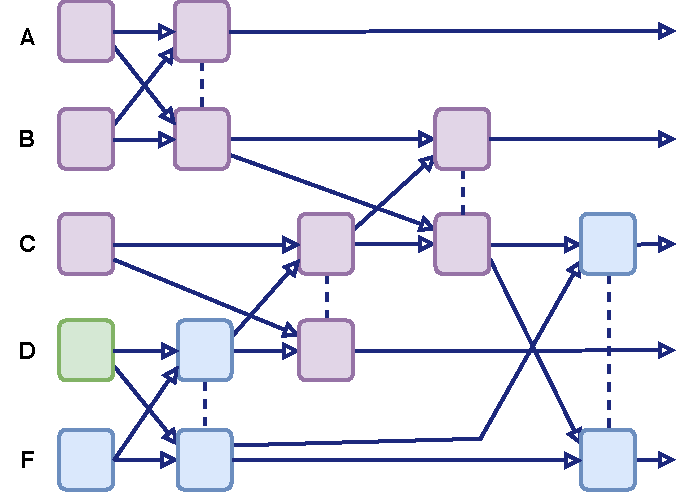
\includegraphics[width=0.5\textwidth]{images/network_state_exchange.pdf}
    \caption{History graph of Network-State-Exchange policy in our model. We again consider 5 agents. The 
    colored blocks show the subjective network state of agent F. The blue blocks are F's own encounters,
    the green block is an encounter received from D while the purple blocks are received from C. This
    time F obtains the complete network state.}
    \label{fig:network_state_exchange}
\end{figure}

The Network-State-Exchange behavior allows any agent $p$ that exchanged information with an agent $q$
to reconstruct the subjective network state of agent $q$ before each interaction. 

% We can define a
% property 

% \begin{defn}[Subjective network state transparency]
%     Given is an ordered encounter model $M = \langle P, I, E, a, w, x \rangle$Let $p$ be an honest agent that applies the Network-State-Exchange policy and let $q$ be an agent
%     that exchanged with $p$. According to Policy \ref{pol:network_state} after a succesful exchange
%     $N_q \subset N_p$ and thus also $H_q \subset N_p$. As previously defined the agent encounter
%     history is a totally ordered set. Let $n_q(t)$ denote the $t$th encounter of agent $q$. At each
%     round $t$ the $q$'s subjective network state is given by $N_q(t) = \{ n \in N : n \in H_p(t-1) \} \cup \{ x(e, p) : e \in E \text{ and } e \in H_p(t-1) \}$.
% \end{defn}

This makes it possible for an honest agent $p$ to re-evaluate $q$'s decisions to engage in each of $q$'s 
interactions.

\begin{thm}[Detectability of verification free-rider]
    \label{thm:ver_free-rider}
    An honest agent who applies the Network-State-Exchange policy is able to repeat all verifications
    of another agent after they exchanged successfully.
\end{thm}
\begin{proof}
    Let $p$ be an honest agent who applies the Network-State-Exchange policy and let $q$ be an agent
    that exchanged with $p$. According to Policy \ref{pol:network_state} after a succesful exchange
    it holds that $N_q \subset N_p$ and thus also $H_q \subset N_p$. As previously defined the agent encounter
    history is a totally ordered set. Let $n_q(t)$ denote the $t$th encounter of agent $q$. At each
    round $t$ the $q$'s subjective network state is given by $N_q(t) = \{ n \in N : n \in H_p(t-1) \} \cup \{ x(e, p) : e \in E \text{ and } e \in H_p(t-1) \}$.
    Also, $N_q(t) \subset N_p$ and therefore $p$ is able to perform Algorithm \ref{alg:verify_exchange}
    for each past transaction of $q$. If for any interaction algorithm $1$ returns false, it is 
    obvious that $q$ did not perform the verification and is therefore a verification free-rider.
\end{proof}

We have shown in Theorem \ref{thm:ver_free-rider} that the Network-State-Exchange policy enables 
agents to effectively find any verification free-rider once that agent's behavior diverges from that
of an honest agent. 

The previous results imply that in a network without any malicious agents a 
verification free-rider cannot be found. 

Also, the question arises who verifies that agents perform this detection of verification 
free-riders. The detection of verification free-riders is a recursive problem and therefore will not
lead to an infinite verification process. However, because agent exchange their complete subjective
network state, they also share their knowledge of malicious agents and free-riders. Suppose an agent
$p$ is aware of a set of malicious agents $S_p$. After exchanging all information with another agent
$q$, $q$'s set of malicious agents should at least contain $S_p \subseteq S_q$. Should an agent $q$ 
interact with any agent in $S_p$, at least agent $p$ knows that $q$ is dishonest. This way $q$ will 
slowly be isolated.

\section{Relevance for global trust system}
\label{sec:relevance}
The calculation of reputation and trust has not been part of the discussion up to now.
This brings about the question of relevance to the global trust system. We refer again to the work
of Otte et. al. \cite{OTTE2017} for an in depth study of interaction graph based trust mechanisms.
The authors show that scoring mechanisms based on a graph representation the interactions between 
agents can be designed to be resilient against Sybil-attacks. For their analysis the authors use the
model stated in Definition \ref{def:old_base} as the basis for creating a graph. We mention in this
section a few conclusions that we can draw from the above theoretical analysis.

\subsection{Manipulation resistance}
Instead of exploring new ways of calculating trust, we analyzed in the above the resilience to of 
the model in the presence of malicious and free riding agents. We have shown that in order to defend
against forks and double spending, information exchange between agents is critical. Only through
ensuring a proper defense against attacks can we warrant the validity of the interactions. Therefore
we create an exchange mechanism that aligns the exchange behavior with an incentive of agents. The
recording of encounters leads to exchange transparency which exposes free-riders. This effectively 
leads to better manipulation resistance and ultimately increases the validity of reputation and 
trust.

\subsection{Increased accuracy of reputation estimate}
Apart from the manipulation resistance, encouraging agents to acquire more data also leads to a
better estimation of the true network state. This in turn leads to more accurate calculation of 
the reputation of peers. According to the model of Mui~\cite{mui2002computational} which was 
introduced Chapter~\ref{chap:problem} this leads to self-reinforcing cycle of more trust and 
increased reciprocity. An analysis of the influence of gossiping on the trust calculation with a
trust mechanism such as the one introduced in \cite{OTTE2017} is an interesting topic for further 
research.

\subsection{Pairwise agreement on reputation}
The Network-State-Exchange policy leads to a synchronization of both agents subjective network state.
After the exchange both agents share the same subjective network state which means they also agree
on the reputation of all peers as the reputation is based on the subjective view of the network.
If trust is calculated with a function that takes as input only the knowledge of reputations or the
records of interactions, both agents can check their trust for each other. This way no dispute can 
exists about the fairness of a trust-based contribution. For example if one agent $p$ is requested by 
two other agents to provide a resource, $p$ cannot falsely donate the resource to the less 
trusted agent in a collusion. The agent who ended up empty handed could prove that the trust 
calculation from $p$'s perspective points in his favor.

\subsection{Reduced scalability}
Enforcing an exchange policy for honest agents also bears risks. An agent is only able to interact
after exchanging some information, in the most stringent case all their knowledge, with another agent. 
This binds a requirement for storage space and bandwidth to the ability of interacting which might 
be too stringent for some application contexts. The costs for an interaction to be possible could 
also lead to local regions of trusted users that share a certain information set. Agents that have
a very similar subjective network state only need to exchange small amounts of data to equalize their
states, thus costs a low. In contrast two agents with completely different sets will need to
exchange large amounts of data. Thus agents with similar information sets are more likely to interact.
On the one hand this can increase the risk of network separation on the other hand this increases 
the difficulty of creating a sybil attacks because only agents with similar information sets can 
act as Sybils which increases their cost.

\subsection{Relation to TrustChain}
The TrustChain can be mapped onto the model defined in this chapter in a straight-forward 
fashion. The blocks store a single transaction and therefore correspond to the interactions of the
model. The functions that relate the interaction to the participating agents and the value of the 
transaction is directly stored on the block itself. The blocks create a fully ordered history of 
each agent. An agents chain then corresponds to the concept of the agent encounter history. Finally, 
the database of blocks that each agent maintains is the subjective network state.

The TrustChain architecture does not define a tool to record the exchange of information. To other 
agents it is not clear which information each agent is acting on. That does not mean that exchange 
is not possible - agents are free to send transaction blocks back and forth. Yet, without recording
this activity, no reward or punishment can be assigned to such behavior or the lack of it. 

\section{Chapter conclusions}
We have shown that exchanging information of interactions and encounters allows to detect a 
fork and double-spend attack. Furthermore, if we can record the exchanges in a similar way as
interactions and make them part of an ordered history, honest agents can ensure that their partners
apply a certain exchange policy. Any agent that does not stick to the policy can be detected and 
dealt with accordingly. 

Finally, if agents apply a strong policy like the Network-State-Exchange policy, agents can
re-evaluate verifications that their peers have done in the past. Any failed verification that still
lead to an interaction will mark agents as lazy verification free-riders or accomplices.